\documentclass[12pt, twoside]{article}
\usepackage{amsmath}
\usepackage{amssymb}
\usepackage[colorlinks=true, linkcolor=black]{hyperref} % Links
\usepackage{makeidx} % Indexierung
\usepackage{siunitx}
\usepackage[english]{babel} % deutsche Sonderzeichen
\usepackage[utf8]{inputenc}
\usepackage{geometry} % Dokumentendesign wie Seiten- oder Zeilenabstand bestimmen
\usepackage[toc,page]{appendix}

% Graphiken
\usepackage{tikz}
\usepackage{pgfplots}
\usepackage{pgfcore}
\usepackage{pgfopts}
\usepackage{pgfornament}
\usepackage{pgf}
\usepackage{ifthen}
\usepackage{booktabs}

% Tabellen
\usepackage{tabu}
\usepackage{longtable}
\usepackage{colortbl} % Tabellen faerben
\usepackage{multirow}
\usepackage{diagbox} % Tabellenzelle diagonal splitten

\usepackage{xcolor} % Farben
\usepackage[framemethod=tikz]{mdframed} % Hintergrunderstellung
\usepackage{enumitem} % Enumerate mit Buchstaben nummerierbar machen
\usepackage{pdfpages}
\usepackage{listings} % Source-Code darstellen
\usepackage{eurosym} % Eurosymbol
\usepackage[square,numbers]{natbib}
\usepackage{here} % figure an richtiger Stelle positionieren
\usepackage{verbatim} % Blockkommentare mit \begin{comment}...\end{comment}
\usepackage{ulem} % \sout{} (durchgestrichener Text)

% BibLaTex
\bibliographystyle{acm}

% Aendern des Anhangnamens (Seite und Inhaltsverzeichnis)
%\renewcommand\appendixtocname{Anhang}
%\renewcommand\appendixpagename{Anhang}

% mdframed Style
\mdfdefinestyle{codebox}{
	linewidth=2.5pt,
	linecolor=codebordercolor,
	backgroundcolor=codecolor,
	shadow=true,
	shadowcolor=black!40!white,
	fontcolor=black,
	everyline=true,
}

% Seitenabstaende
\geometry{left=15mm,right=15mm,top=15mm,bottom=20mm}

% TikZ Bibliotheken
\usetikzlibrary{
    arrows,
    arrows.meta,
    decorations,
    backgrounds,
    positioning,
    fit,
    petri,
    shadows,
    datavisualization.formats.functions,
    calc,
    shapes,
    shapes.multipart
}

\pgfplotsset{width=7cm,compat=1.15}

\definecolor{codecolor}{HTML}{EEEEEE}
\definecolor{codebordercolor}{HTML}{CCCCCC}

% Standardeinstellungen fuer Source-Code
\lstset{
    language=C,
    breaklines=true,
    keepspaces=true,
    keywordstyle=\bfseries\color{green!70!black},
    basicstyle=\ttfamily\color{black},
    commentstyle=\itshape\color{purple},
    identifierstyle=\color{blue},
    stringstyle=\color{orange},
    showstringspaces=false,
    rulecolor=\color{black},
    tabsize=2,
    escapeinside={\%*}{*\%},
}

%
% Tikz-library for UML
%

% Arrow tips {{{

  % umlaggreg {{{
  \tikzset{
    umlaggreg /.tip = {Diamond[fill=white,scale=1.75]}
  }
  % }}}

  % umlcompo {{{
  \tikzset{
    umlcompo /.tip = {Diamond[fill=black,scale=1.75]}
  }
  % }}}

  % umlgeneral {{{
  \tikzset{
    umlgeneral /.tip = {Triangle[fill=white,scale=1.75]}
  }
  % }}}

  % umlportprovider {{{
  \tikzset{
    umlportprovider /.tip = {Circle[
      length=8pt,
      width=8pt,
      fill=white
    ]}
  }
  % }}}

  % umlportproviderREST {{{
  \tikzset{
    umlportproviderREST /.tip = {Circle[
      length=8pt,
      width=8pt,
      fill=blue
    ]}
  }
  % }}}

  % umlportproviderEvent {{{
  \tikzset{
    umlportproviderEvent /.tip = {Circle[
      length=8pt,
      width=8pt,
      fill=red
    ]}
  }
  % }}}

  % umlportcaller {{{
  \tikzset{
    umlportcaller /.tip = {Arc Barb[
      reversed,
      length=3pt,
      width=8pt
    ]}
  }
  % }}}

% }}}

% Use-case {{{
\tikzset{
  usecase/.style={
    ellipse,
    fill=blue!20,
    align=center,
    draw
  }
}
% }}}

%%%%%%%%%%%%%%%%%%%%%%%%%%%%%%%%%%%%%%%%%%%%%%%%%%%%%%%%%%%%%%%%%%%%%%%%%%%%%%%%%%%%%%%%%%%%%%%%%%%%%%%%%%%%%%%%%%%%%%%%%%%%%%%%%%%%%%%%%%%%%%%%%%
%UML Component Token
%%%%%%%%%%%%%%%%%%%%%%%%%%%%%%%%%%%%%%%%%%%%%%%%%%%%%%%%%%%%%%%%%%%%%%%%%%%%%%%%%%%%%%%%%%%%%%%%%%%%%%%%%%%%%%%%%%%%%%%%%%%%%%%%%%%%%%%%%%%%%%%%%%
\def\UMLComponentToken#1#2#3{
	\draw [#3]($(#1.north east)-(0.1,0.1)$) rectangle ($(#1.north east)-(0.3,0.45)$);
	\draw [#3,fill=#2]($(#1.north east)-(0.35,0.2)$) rectangle ($(#1.north east)-(0.25,0.25)$);
	\draw [#3,fill=#2]($(#1.north east)-(0.35,0.3)$) rectangle ($(#1.north east)-(0.25,0.35)$);
}

%%%%%%%%%%%%%%%%%%%%%%%%%%%%%%%%%%%%%%%%%%%%%%%%%%%%%%%%%%%%%%%%%%%%%%%%%%%%%%%%%%%%%%%%%%%%%%%%%%%%%%%%%%%%%%%%%%%%%%%%%%%%%%%%%%%%%%%%%%%%%%%%%%
%UML Component
%%%%%%%%%%%%%%%%%%%%%%%%%%%%%%%%%%%%%%%%%%%%%%%%%%%%%%%%%%%%%%%%%%%%%%%%%%%%%%%%%%%%%%%%%%%%%%%%%%%%%%%%%%%%%%%%%%%%%%%%%%%%%%%%%%%%%%%%%%%%%%%%%%
%USAGE:
% 	\UMLComponent{name}{width}{height}{Position eines Ports und Beschreibender UMLNote in der Form:
%																				positionPort/noteX/noteY/noteText/noteColor
%
%BEISPIEL:
%		\UMLComponent{Bestellvorgang}{\linewidth-0.2cm}{15cm}{
%			Bestellvorgang.east/7/1.5/Bestellvorgang ausf\"uhren/yellow!25,
%			Bestellvorgang.south/-2/-6/Blah/yellow!25,
%			Bestellvorgang.310/7/-6/Blahhh/yellow!25
%		}
\def\UMLComponent#1#2#3#4{
	\node [rectangle split, rectangle split parts = 2,rectangle split empty part height=#3,draw,fill=yellow!25,inner ysep=7pt,inner xsep=15pt,minimum size=#2] at(0,0) (#1) {#1 \nodepart{second}};
	\UMLComponentToken{#1}{yellow!25}{}
	\foreach \port/\notex/\notey/\notetext/\notecolor in {#4}{
		\UMLNote{\notex}{\notey}{\notetext}{\port}{\notecolor};
		\draw[fill=yellow!25] ($(\port) - (.2,.2)$) rectangle ($(\port)+(.2,.2)$);
	};
}

% UML Simple Component {{{

% 1. x
% 2. y
% 3. text/name
% 4. options
\def\UMLSComponent#1#2#3#4{
	\node[
    rectangle split,
    rectangle split parts = 2,
    rectangle split empty part height=1cm,
    draw,
    fill=yellow!25,
    inner ysep=7pt,
    inner xsep=15pt,
    #4
  ] at(#1,#2) (#3) {#3 \nodepart{second}};
	\UMLComponentToken{#3}{yellow!25}{}
}

% 1. Relative to
% 2. Text/Name
% 3. Options
\def\UMLSComponentRelativeTo#1#2#3{
	\node[
    rectangle split,
    rectangle split parts = 2,
    rectangle split empty part height=1cm,
    draw,
    fill=yellow!25,
    inner ysep=7pt,
    inner xsep=15pt,
    #1,
    #3
  ] (#2) {#2 \nodepart{second}};
	\UMLComponentToken{#2}{yellow!25}{}
}

% 1. Relative to
% 2. Text
% 3. Name
% 4. Options
\def\UMLSComponentRelativeToAlterName#1#2#3#4{
	\node[
    rectangle split,
    rectangle split parts = 2,
    rectangle split empty part height=1cm,
    draw,
    fill=yellow!25,
    inner ysep=7pt,
    inner xsep=15pt,
    #1,
    #4
  ] (#3) {#2 \nodepart{second}};
	\UMLComponentToken{#3}{yellow!25}{}
}

% 1. Relative to
% 2. Text
% 3. Name
% 4. Options
\def\UMLSComponentRelativeToAlterName#1#2#3#4{
	\node [rectangle split, rectangle split parts = 2,rectangle split empty part height=1cm,draw, fill=yellow!25,inner ysep=7pt,inner xsep=15pt,#1,#4](#3) {#2 \nodepart{second}};
	\UMLComponentToken{#3}{yellow!25}{}
}

% }}}

%%%%%%%%%%%%%%%%%%%%%%%%%%%%%%%%%%%%%%%%%%%%%%%%%%%%%%%%%%%%%%%%%%%%%%%%%%%%%%%%%%%%%%%%%%%%%%%%%%%%%%%%%%%%%%%%%%%%%%%%%%%%%%%%%%%%%%%%%%%%%%%%%%
%UML Extern Component
%%%%%%%%%%%%%%%%%%%%%%%%%%%%%%%%%%%%%%%%%%%%%%%%%%%%%%%%%%%%%%%%%%%%%%%%%%%%%%%%%%%%%%%%%%%%%%%%%%%%%%%%%%%%%%%%%%%%%%%%%%%%%%%%%%%%%%%%%%%%%%%%%%
\def\UMLExternComponent#1#2#3{
	\node [rectangle split, rectangle split parts = 2,rectangle split empty part height=1cm,draw, fill=black!10,inner ysep=7pt,inner xsep=15pt] at(#1,#2) (#3) {$<<$#3$>>$ \nodepart{second}};
	\UMLComponentToken{#3}{black!10}{}
}

%%%%%%%%%%%%%%%%%%%%%%%%%%%%%%%%%%%%%%%%%%%%%%%%%%%%%%%%%%%%%%%%%%%%%%%%%%%%%%%%%%%%%%%%%%%%%%%%%%%%%%%%%%%%%%%%%%%%%%%%%%%%%%%%%%%%%%%%%%%%%%%%%%
%UML Note
%%%%%%%%%%%%%%%%%%%%%%%%%%%%%%%%%%%%%%%%%%%%%%%%%%%%%%%%%%%%%%%%%%%%%%%%%%%%%%%%%%%%%%%%%%%%%%%%%%%%%%%%%%%%%%%%%%%%%%%%%%%%%%%%%%%%%%%%%%%%%%%%%%
%USAGE:
%	\UMLNote{x}{y}{text}{to (--)}{color (rectangle north east)}
\def\UMLNote#1#2#3#4#5{
	\node [rectangle,fill=green!25,draw,inner ysep=15pt,inner xsep=6pt,text width=3cm] at (#1,#2) (b) {\small{#3}};
	\draw [fill=#5,#5]($(b.north east) + (.1,.1)$) -- ($(b.north east) - (0,.5)$) -- ($(b.north east) - (.5,0)$) -- cycle;
	\draw ($(b.north east) - (.01,.5)$) -- ($(b.north east) - (.5,.01)$) -- ($(b.north east)-(.5,.5)$) -- cycle;
	\draw [dashed](b) -- (#4);
}

%%%%%%%%%%%%%%%%%%%%%%%%%%%%%%%%%%%%%%%%%%%%%%%%%%%%%%%%%%%%%%%%%%%%%%%%%%%%%%%%%%%%%%%%%%%%%%%%%%%%%%%%%%%%%%%%%%%%%%%%%%%%%%%%%%%%%%%%%%%%%%%%%%
% UML Component Port
%%%%%%%%%%%%%%%%%%%%%%%%%%%%%%%%%%%%%%%%%%%%%%%%%%%%%%%%%%%%%%%%%%%%%%%%%%%%%%%%%%%%%%%%%%%%%%%%%%%%%%%%%%%%%%%%%%%%%%%%%%%%%%%%%%%%%%%%%%%%%%%%%%

% 1. position
% 2. options (draw)
\def\UMLComponentPort#1#2{
	\draw[fill=yellow!25,#2] ($(#1)-(.2,.2)$) rectangle ($(#1)+(.2,.2)$);
}

%%%%%%%%%%%%%%%%%%%%%%%%%%%%%%%%%%%%%%%%%%%%%%%%%%%%%%%%%%%%%%%%%%%%%%%%%%%%%%%%%%%%%%%%%%%%%%%%%%%%%%%%%%%%%%%%%%%%%%%%%%%%%%%%%%%%%%%%%%%%%%%%%%
% UML Component Connector with Ports on both ends
%%%%%%%%%%%%%%%%%%%%%%%%%%%%%%%%%%%%%%%%%%%%%%%%%%%%%%%%%%%%%%%%%%%%%%%%%%%%%%%%%%%%%%%%%%%%%%%%%%%%%%%%%%%%%%%%%%%%%%%%%%%%%%%%%%%%%%%%%%%%%%%%%%
\def\UMLComponentPortConnector#1#2#3#4#5#6#7#8{
	\draw[#3,-{>[sep=3.5]>}] (#1) #4 (#2);
	\UMLNote{#5}{#6}{#7}{#2}{#8}
	\draw[fill=yellow!25] ($(#1)-(.2,.2)$) rectangle ($(#1)+(.2,.2)$);
	\draw[fill=yellow!25] ($(#2)-(.2,.2)$) rectangle ($(#2)+(.2,.2)$);
}

%%%%%%%%%%%%%%%%%%%%%%%%%%%%%%%%%%%%%%%%%%%%%%%%%%%%%%%%%%%%%%%%%%%%%%%%%%%%%%%%%%%%%%%%%%%%%%%%%%%%%%%%%%%%%%%%%%%%%%%%%%%%%%%%%%%%%%%%%%%%%%%%%%
% UML Component Realizor with Ports on both ends
%%%%%%%%%%%%%%%%%%%%%%%%%%%%%%%%%%%%%%%%%%%%%%%%%%%%%%%%%%%%%%%%%%%%%%%%%%%%%%%%%%%%%%%%%%%%%%%%%%%%%%%%%%%%%%%%%%%%%%%%%%%%%%%%%%%%%%%%%%%%%%%%%%
\def\UMLComponentPortRealizor#1#2#3#4#5#6#7#8{
	\draw[#3,-{Stealth[sep=3.5,inset=0pt,length=5pt,width=5pt]>},blue] (#1) #4 (#2);
	\UMLNote{#5}{#6}{#7}{#2}{#8}
	\draw[fill=yellow!25] ($(#1)-(.2,.2)$) rectangle ($(#1)+(.2,.2)$);
	\draw[fill=yellow!25] ($(#2)-(.2,.2)$) rectangle ($(#2)+(.2,.2)$);
}

% UML Class (various) {{{
%
% 1. Normal                         -> \UMLClass { X } { Y } { Text/Name } { Options (node) }
% 2. Normal mit alternativem Namen  -> \UMLClassAlterName { X } { Y } { Text } { Name } { Options (node) }
% 3. Relativ                        -> \UMLClassRelativeTo { Relative to } { Text/Name } { Options (node) }
% 4. Relativ mit alternativem Namen -> \UMLClassRelativeToAlterName { Relative to } { Text } { Name } { Options (node) }

  % 1. Normal {{{
  \def\UMLClass#1#2#3#4{
    \node [
      fill = yellow!25,
      rectangle split,
      rectangle split parts = 3,
      rectangle split ignore empty parts = true,
      rectangle split part align = {center, left, left},
      inner xsep = 15pt,
      inner ysep = 7pt,
      draw,
      #4
    ] at(#1,#2) (#3) {#3};
  }
  % }}}

  % 2. Normal mit alternativem Namen {{{
    \def\UMLClassAlterName#1#2#3#4#5{
      \node [
        fill = yellow!25,
        rectangle split,
        rectangle split parts = 3,
        rectangle split ignore empty parts = true,
        rectangle split part align = {center, left, left},
        inner xsep = 15pt,
        inner ysep = 7pt,
        draw,
        #5
      ] at (#1, #2) (#4) {#3};
    }
  % }}}

  % 3. Relativ {{{
    \def\UMLClassRelativeTo#1#2#3{
      \node [
        fill = yellow!25,
        rectangle split,
        rectangle split parts = 3,
        rectangle split ignore empty parts = true,
        rectangle split part align = {center, left, left},
        inner xsep = 15pt,
        inner ysep = 7pt,
        draw,
        #1,
        #3
      ] (#2) {#2};
    }
  % }}}

  % 4. Relativ {{{
    \def\UMLClassRelativeToAlterName#1#2#3#4{
      \node [
        fill = yellow!25,
        rectangle split,
        rectangle split parts = 3,
        rectangle split ignore empty parts = true,
        rectangle split part align = {center, left, left},
        inner xsep = 15pt,
        inner ysep = 7pt,
        draw,
        #1,
        #4
      ] (#3) {#2};
    }
  % }}}

% }}}

% UML Actor (various) {{{
%
% 1. Normal
%    -> \UMLActor { X } { Y } { Text/Name }
% 2. Normal mit alternativem Namen
%    -> \UMLActorAlterName { X } { Y } { Text } { Name }
% 3. Relativ
%    -> \UMLActorRelativeTo { Relative to } { Text/Name }
% 4. Relativ mit alternativem Namen
%    -> \UMLActorRelativeToAlterName { Relative to } { Text } { Name }

  % DrawActor {{{
  \def\DrawActor#1{

    % Body {{{
    \draw[scale=.5] ($(#1)+(0,.5)$) -- ($(#1)-(0,.5)$);
    % }}}

    % Left leg {{{
    \draw[scale=.5] ($(#1)-(0,.5)$) -- ($(#1)+(.5,-1)$);
    % }}}

    % Right leg {{{
    \draw[scale=.5] ($(#1)-(0,.5)$) -- ($(#1)+(-.5,-1)$);
    % }}}

    % Arms {{{
    \draw[scale=.5] ($(#1)+(.5,.25)$) -- ($(#1)+(-.5,.25)$);
    % }}}

    % Head {{{
    \draw[scale=.5] ($(#1)+(0,.75)$) circle (.25);
    % }}}

  }
  % }}}

  % 1. Normal {{{
  \def\UMLActor#1#2#3{

    % Node for referencing actor {{{
    \node[
      label=below:#3,
      inner ysep=.55cm,
      inner xsep=.3cm
    ] at (#1,#2) (#3) {};
    % }}}

    \DrawActor{#3}

  }
  % }}}

  % 2. Normal mit alternativem Namen {{{
  \def\UMLActorAlterName#1#2#3#4{

    % Node for referencing actor {{{
    \node[
      label=below:#3,
      inner ysep=.55cm,
      inner xsep=.3cm
    ] at (#1,#2) (#4) {};
    % }}}

    \DrawActor{#4}

  }
  % }}}

  % 3. Relativ {{{
  \def\UMLActorRelativeTo#1#2{

    % Node for referencing actor {{{
    \node[
      label=below:#2,
      inner ysep=.55cm,
      inner xsep=.3cm,
      #1
    ] (#2) {};
    % }}}

    \DrawActor{#2}

  }
  % }}}

  % 4. Relativ {{{
  \def\UMLActorRelativeToAlterName#1#2#3{

    % Node for referencing actor {{{
    \node[
      label=below:#2,
      inner ysep=.55cm,
      inner xsep=.3cm,
      #1
    ] (#3) {};
    % }}}

    \DrawActor{#3}

  }
  % }}}

% }}}

%
% UML Activity State (various)
%
% 1. Normal                         -> \UMLActivityState{ X }{ Y }{ Text/Name }{ Options (node) }
% 2. Normal mit alternativem Namen  -> \UMLActivityStateAlterName{ X }{ Y }{ Text }{ Name }{ Options (node) }
% 3. Relativ                        -> \UMLActivityStateRelativeTo{ Relative to }{ Text/Name }{ Options (node) }
% 4. Relativ mit alternativem Namen -> \UMLActivityStateRelativeToAlterName{ Relative to }{ Text }{ Name }{ Options (node) }
%
%

% 1. Normal
%
% #1: X
% #2: Y
% #3: Text/Name
% #4: Options (node)

\def\UMLActivityState#1#2#3#4{
	\node [rectangle,rounded corners,draw,fill=black!10,inner ysep=9pt,inner xsep=22pt,#4] at(#1,#2) (#3) {#3};
	\UMLActivityStateToken{#3}
}

% 2. Alternativer Name
%
% #1: X
% #2: Y
% #3: Text
% #4: Name
% #5: Options (node)

\def\UMLActivityStateAlterName#1#2#3#4#5{
	\node [rectangle,rounded corners,draw,fill=black!10,inner ysep=9pt,inner xsep=22pt,#5] at(#1,#2) (#4) {#3};
	\UMLActivityStateToken{#4}
}


% 3. Relativ
%
% #1: Relative to (z.B. below=1 of ...)
% #2: Text/Name
% #3: Options (node)

\def\UMLActivityStateRelativeTo#1#2#3{
	\node [rectangle,rounded corners,draw,fill=black!10,inner ysep=9pt,inner xsep=22pt,#1,#3] (#2) {#2};
	\UMLActivityStateToken{#2}
}


% 4. Relativ mit alternativem Namen
%
% #1: Relative to (z.B. below=1 of ...)
% #2: Text
% #3: Name
% #4: Options

\def\UMLActivityStateRelativeToAlterName#1#2#3#4{
	\node [rectangle,rounded corners,draw,fill=black!10,inner ysep=9pt,inner xsep=22pt,#1,#4] (#3) {#2};
	\UMLActivityStateToken{#3}
}


% Token

\def\UMLActivityStateToken#1{
	\draw[fill=yellow!25,rounded corners] ($(#1.west)+(.3,.25)$) rectangle ($(#1.west)+(.7,-.15)$);
}


%
% UML Activity Object (various)
%
% 1. Normal                         -> \UMLActivityObject{ X }{ Y }{ Text/Name }{ Options (node) }
% 2. Normal mit alternativem Namen  -> \UMLActivityObjectAlterName{ X }{ Y }{ Text }{ Name }{ Options (node) }
% 3. Relativ                        -> \UMLActivityObjectRelativeTo{ Relative to }{ Text/Name }{ Options (node) }
% 4. Relativ mit alternativem Namen -> \UMLActivityObjectRelativeToAlterName{ Relative to }{ Text }{ Name }{ Options (node) }
%
%

% 1. Normal
%
% #1: X
% #2: Y
% #3: Text/Name
% #4: Options (node)

\def\UMLActivityObject#1#2#3#4{
	\node [rectangle,draw,fill=green!15,inner ysep=9pt,inner xsep=25pt,#4] at(#1,#2) (#3) {:#3};
	\UMLActivityObjectToken{#3}
}


% 2. Alternativer Name
%
% #1: X
% #2: Y
% #3: Text
% #4: Name
% #5: Options (node)

\def\UMLActivityObjectAlterName#1#2#3#4#5{
	\node [rectangle,draw,fill=green!15,inner ysep=9pt,inner xsep=25pt,#5] at(#1,#2) (#4) {:#3};
	\UMLActivityObjectToken{#4}
}


% 3. Relativ
%
% #1: Relative to (z.B. below=1 of ...)
% #2: Text/Name
% #3: Options (node)

\def\UMLActivityObjectRelativeTo#1#2#3{
	\node [rectangle,draw,fill=green!15,inner ysep=9pt,inner xsep=25pt,#3,#1] (#2) {:#2};
	\UMLActivityObjectToken{#2}
}


% 4. Relativ mit alternativem Namen
%
% #1: Relative to (z.B. below=1 of ...)
% #2: Text
% #3: Name
% #4: Options

\def\UMLActivityObjectRelativeToAlterName#1#2#3#4{
	\node [rectangle,draw,fill=green!15,inner ysep=9pt,inner xsep=25pt,#4,#1] (#3) {:#2};
	\UMLActivityObjectToken{#3}
}


% Token

\def\UMLActivityObjectToken#1{
	\draw[fill=yellow!25] ($(#1.west)+(.3,.25)$) rectangle ($(#1.west)+(.7,.11)$);
	\draw ($(#1.west)+(.35,.18)$) -- ($(#1.west)+(.65,.18)$);
	\draw[fill=yellow!25] ($(#1.west)+(.3,.11)$) rectangle ($(#1.west)+(.7,-.02)$);
	\draw[fill=yellow!25] ($(#1.west)+(.3,-.02)$) rectangle ($(#1.west)+(.7,-.15)$);
}


%
% UML Activity Data Storage (various)
%
% 1. Normal                         -> \UMLActivityDataStorage{ X }{ Y }{ Text/Name }{ Options (node) }
% 2. Normal mit alternativem Namen  -> \UMLActivityDataStorageAlterName{ X }{ Y }{ Text }{ Name }{ Options (node) }
% 3. Relativ                        -> \UMLActivityDataStorageRelativeTo{ Relative to }{ Text/Name }{ Options (node) }
% 4. Relativ mit alternativem Namen -> \UMLActivityDataStorageRelativeToAlterName{ Relative to }{ Text }{ Name }{ Options (node) }
%
%

% 1. Normal
%
% #1: X
% #2: Y
% #3: Text/Name
% #4: Options (node)

\def\UMLActivityDataStorage#1#2#3#4{
	\node [rectangle,draw,fill=green!15,inner ysep=9pt,inner xsep=25pt,#4] at(#1,#2) (#3) {#3};
	\UMLActivityDataStorageToken{#3}
}


% 2. Alternativer Name
%
% #1: X
% #2: Y
% #3: Text
% #4: Name
% #5: Options (node)

\def\UMLActivityDataStorageAlterName#1#2#3#4#5{
	\node [rectangle,draw,fill=green!15,inner ysep=9pt,inner xsep=25pt,#5] at(#1,#2) (#4) {#3};
	\UMLActivityDataStorageToken{#4}
}


% 3. Relativ
%
% #1: Relative to (z.B. below=1 of ...)
% #2: Text/Name
% #3: Options (node)

\def\UMLActivityDataStorageRelativeTo#1#2#3{
	\node [rectangle,draw,fill=green!15,inner ysep=9pt,inner xsep=25pt,#3,#1] (#2) {#2};
	\UMLActivityDataStorageToken{#2}
}


% 4. Relativ mit alternativem Namen
%
% #1: Relative to (z.B. below=1 of ...)
% #2: Text
% #3: Name
% #4: Options

\def\UMLActivityDataStorageRelativeToAlterName#1#2#3#4{
	\node [rectangle,draw,fill=green!15,inner ysep=9pt,inner xsep=25pt,#4,#1] (#3) {#2};
	\UMLActivityDataStorageToken{#3}
}


% Token

\def\UMLActivityDataStorageToken#1{
	\node[rectangle,draw,scale=.5,fill=yellow!25] at($(#1.west)+(.5,-.05)$) (ds) {DS};
	\draw[-{>[scale width=.5]}] ($(ds.north west)+(0,.15)$) -| (ds.north);
	\draw[-{>[scale width=.5]}] (ds.east) -- ($(ds.east)+(.15,0)$);
}


%
% UML Activity Central Buffer (various)
%
% 1. Normal                         -> \UMLActivityCentralBuffer{ X }{ Y }{ Text/Name }{ Options (node) }
% 2. Normal mit alternativem Namen  -> \UMLActivityCentralBufferAlterName{ X }{ Y }{ Text }{ Name }{ Options (node) }
% 3. Relativ                        -> \UMLActivityCentralBufferRelativeTo{ Relative to }{ Text/Name }{ Options (node) }
% 4. Relativ mit alternativem Namen -> \UMLActivityCentralBufferRelativeToAlterName{ Relative to }{ Text }{ Name }{ Options (node) }
%
%

% 1. Normal
%
% #1: X
% #2: Y
% #3: Text/Name
% #4: Options (node)

\def\UMLActivityCentralBuffer#1#2#3#4{
	\node [rectangle,draw,fill=green!15,inner ysep=9pt,inner xsep=25pt,#4] at(#1,#2) (#3) {#3};
	\UMLActivityCentralBufferToken{#3}
}


% 2. Alternativer Name
%
% #1: X
% #2: Y
% #3: Text
% #4: Name
% #5: Options (node)

\def\UMLActivityCentralBufferAlterName#1#2#3#4#5{
	\node [rectangle,draw,fill=green!15,inner ysep=9pt,inner xsep=25pt,#5] at(#1,#2) (#4) {#3};
	\UMLActivityCentralBufferToken{#4}
}


% 3. Relativ
%
% #1: Relative to (z.B. below=1 of ...)
% #2: Text/Name
% #3: Options (node)

\def\UMLActivityCentralBufferRelativeTo#1#2#3{
	\node [rectangle,draw,fill=green!15,inner ysep=9pt,inner xsep=25pt,#3,#1] (#2) {#2};
	\UMLActivityCentralBufferToken{#2}
}


% 4. Relativ mit alternativem Namen
%
% #1: Relative to (z.B. below=1 of ...)
% #2: Text
% #3: Name
% #4: Options

\def\UMLActivityCentralBufferRelativeToAlterName#1#2#3#4{
	\node [rectangle,draw,fill=green!15,inner ysep=9pt,inner xsep=25pt,#4,#1] (#3) {#2};
	\UMLActivityCentralBufferToken{#3}
}


% Token

\def\UMLActivityCentralBufferToken#1{
	\node[rectangle,draw,scale=.5,fill=yellow!25] at($(#1.west)+(.5,-.05)$) (cb) {CB};
	\draw[-{>[scale width=.5]}] ($(cb.north west)+(0,.15)$) -| (cb.north);
	\draw[-{>[scale width=.5]}] (cb.east) -- ($(cb.east)+(.15,0)$);
}


% 1. N1
% 2. N2
% 3. Path
\def\UMLActivityControlFlow#1#2#3{
	\draw[blue,->] (#1) #3 (#2);
}

% 1. N1
% 2. N2
% 3. Path
% 4. Text
% 5. Text Pos
% 6. Text Options
\def\UMLActivityControlFlowWithGuard#1#2#3#4#5#6{
	\draw[blue,->] (#1) #3 (#2);
	\node[#6] at ($(#1)!#5!(#2)$) {\tiny{[#4]}};
}

% 1. N1
% 2. N2
% 3. Path
% 4. Text
% 5. Text Pos
% 6. Text Options
\def\UMLActivityControlFlowWithText#1#2#3#4#5#6{
	\draw[blue,->] (#1) #3 (#2);
	\node[#6] at ($(#1)!#5!(#2)$) {\tiny{#4}};
}



% UML Activity Data Flow (various)

\def\UMLActivityDataFlowPort#1#2#3{
	\draw[fill=#3] ($(#1)-(.15,.15)$) rectangle ($(#1)+(.15,.15)$);
	\draw[->,rotate=#2] ($(#1)-(.1,0)$) -- ($(#1)+(.1,0)$);
}

\def\UMLActivityDataFlow#1#2#3#4#5{
	\draw[brown!50!black,-{>[sep=3pt]>}] (#1) #3 (#2);
	\UMLActivityDataFlowPort{#1}{#4}{blue!25}
	\UMLActivityDataFlowPort{#2}{#5}{orange!25}
}

% 1. N1
% 2. N2
% 3. Path
% 4. Text
% 5. Text Options N1
% 6. Text Options N2
% 7. Arrow Direction (Deg) N1
% 8. Arrow Direction (Deg) N2

\def\UMLActivityDataFlowWithText#1#2#3#4#5#6#7#8{
	\draw[brown!50!black,-{>[sep=3pt]>}] (#1) #3 (#2);
	\node[#5] at (#1) {\tiny{#4}};
	\node[#6] at (#2) {\tiny{#4}};
	\UMLActivityDataFlowPort{#1}{#7}{blue!25}
	\UMLActivityDataFlowPort{#2}{#8}{orange!25}
}

\def\UMLActivityDataFlowNoPorts#1#2#3{
	\draw[brown!50!black,->] (#1) #3 (#2);
}

\def\UMLActivityDataFlowIn#1#2#3#4{
	\draw[brown!50!black,-{>[sep=3pt]>}] (#1) #3 (#2);
	\UMLActivityDataFlowPort{#2}{#4}{orange!25}
}

% 1. N1
% 2. N2
% 3. Path
% 4. Text
% 5. Text Pos
% 6. Text Options
% 7. Arrow Direction (Deg)

\def\UMLActivityDataFlowInWithText#1#2#3#4#5#6#7{
	\draw[brown!50!black,-{>[sep=3pt]>}] (#1) #3 (#2);
	\node[#6] at ($(#1)!#5!(#2)$) {\tiny{#4}};
	\UMLActivityDataFlowPort{#2}{#7}{orange!25}
}

\def\UMLActivityDataFlowOut#1#2#3#4{
	\draw[brown!50!black,->] (#1) #3 (#2);
	\UMLActivityDataFlowPort{#1}{#4}{blue!25}
}

\def\UMLActivityDataFlowOutWithText#1#2#3#4#5#6#7{
	\draw[brown!50!black,->] (#1) #3 (#2);
	\node[#6] at ($(#1)!#5!(#2)$) {\tiny{#4}};
	\UMLActivityDataFlowPort{#1}{#7}{blue!25}
}


% Nodes

\def\UMLActivityInitialNode#1#2{
	\node[circle,draw,inner sep=5pt,fill=black] at (#1,#2) (initial) {};
}

\def\UMLActivityInitialNodeRelativeTo#1{
	\node[circle,draw,inner sep=5pt,fill=black,#1] (initial) {};
}

\def\UMLActivityFinalNode#1#2#3{
	\draw[fill=black] (#1,#2) circle (.2cm);
	\node[circle,draw,inner sep=5pt] at (#1,#2) (#3) {};
}

\def\UMLActivityFinalNodeRelativeTo#1#2{
	\node[circle,draw,inner sep=5pt,#1] (#2) {};
	\node[circle,draw,inner sep=4pt,fill=black] at (#2) {};
}

\def\UMLActivityExitNode#1#2#3{
	\node[circle,draw,fill=white,inner sep=5pt] at (#1,#2) (#3) {};
	\draw (#3.north west) -- (#3.south east);
	\draw (#3.north east) -- (#3.south west);
}

\def\UMLActivityExitNodeRelativeTo#1#2{
	\node[circle,draw,fill=white,inner sep=5pt,#1] (#2) {};
	\draw (#2.north west) -- (#2.south east);
	\draw (#2.north east) -- (#2.south west);
}

\def\UMLActivityDescisionNode#1#2#3{
	\node[diamond,draw,fill=black!10,aspect=.75] at (#1,#2) (#3) {};
}

\def\UMLActivityDescisionNodeRelativeTo#1#2{
	\node[diamond,draw,fill=black!10,aspect=.75,#1] (#2) {};
}

% 1. Relative to
% 2. Name
% 3. Text
% 4. Text Options
\def\UMLActivityWaitTimeActionRelativeTo#1#2#3#4#5{
	\node[#1,minimum size=.5cm] (#2) {};
	\node[#5] at (#4) {\tiny{#3}};
	\draw ($(#2) - (.25,.25)$) -- ($(#2) + (.25,.25)$) -- ($(#2) + (-.25,.25)$) -- ($(#2) + (.25,-.25)$) -- cycle;
	%\node[isosceles triangle,draw,#1,rotate=90,below left] (#2_bottom) {};
}

% 1. X
% 2. Y
% 3. Name
% 4. Size
\def\UMLActivityConcurrentNodeH#1#2#3#4{
	\node[rectangle,draw,fill=black,inner ysep=1pt,inner xsep=#4/2] at (#1,#2) (#3) {};
}

% 1. Relative to
% 2. Name
% 3. Size
\def\UMLActivityConcurrentNodeHRelativeTo#1#2#3{
	\node[rectangle,draw,fill=black,inner ysep=1pt,inner xsep=#3/2,#1] (#2) {};
}

% 1. X
% 2. Y
% 3. Name
% 4. Size
\def\UMLActivityConcurrentNodeV#1#2#3#4{
	\node[rectangle,draw,fill=black,inner xsep=1pt,inner ysep=#4/2] at (#1,#2) (#3) {};
}

% 1. Relative to
% 2. Name
% 3. Size
% 4. Options
\def\UMLActivityConcurrentNodeVRelativeTo#1#2#3#4{
	\node[rectangle,draw,fill=black,inner xsep=1pt,inner ysep=#3/2,#1,#4] (#2) {};
}

\def\UMLActivitySwimlane#1#2#3#4{
	\node[black!25,rectangle split, rectangle split parts = 2,rectangle split empty part height=#3,draw,fill=yellow!10,inner ysep=7pt,inner xsep=15pt,minimum size=#2,#4] (#1) {#1 \nodepart{second}};
	\UMLComponentToken{#1}{yellow!10}{black!25}
}

\def\UMLActivityExternSwimlane#1#2#3#4{
	\node [black!25,rectangle split, rectangle split parts = 2,draw,fill=black!5,inner ysep=7pt,inner xsep=15pt,rectangle split empty part height=#3,minimum size=#2,#4] (#1) {#1 \nodepart{second}};
	\UMLComponentToken{#1}{black!5}{black!25}
}

%%%%%%%%%%%%%%%%%%%%%%%%%%%%%%%%%%%%%%%%%%%%%%%%%%%%%%%%%%%%%%%%%%%%%%%%%%
% State Diagram
%%%%%%%%%%%%%%%%%%%%%%%%%%%%%%%%%%%%%%%%%%%%%%%%%%%%%%%%%%%%%%%%%%%%%%%%%
%
% UML State Diagramm Object State (various)
%
% 1. Normal                         -> \UMLActivityState{ X }{ Y }{ Text/Name }{ Options (node) }
% 2. Normal mit alternativem Namen  -> \UMLActivityStateAlterName{ X }{ Y }{ Text }{ Name }{ Options (node) }
% 3. Relativ                        -> \UMLActivityStateRelativeTo{ Relative to }{ Text/Name }{ Options (node) }
% 4. Relativ mit alternativem Namen -> \UMLActivityStateRelativeToAlterName{ Relative to }{ Text }{ Name }{ Options (node) }
%
%

% 1. Normal
%
% #1: X
% #2: Y
% #3: Text/Name
% #4: Options (node)

\def\UMLStateObjectState#1#2#3#4{
	\node [rectangle,rounded corners,draw,fill=black!10,inner ysep=9pt,inner xsep=10pt,#4] at(#1,#2) (#3) {#3};
}

% 2. Alternativer Name
%
% #1: X
% #2: Y
% #3: Text
% #4: Name
% #5: Options (node)

\def\UMLStateObjectStateAlterName#1#2#3#4#5{
	\node [rectangle,rounded corners,draw,fill=black!10,inner ysep=9pt,inner xsep=10pt,#5] at(#1,#2) (#4) {#3};
}


% 3. Relativ
%
% #1: Relative to (z.B. below=1 of ...)
% #2: Text/Name
% #3: Options (node)

\def\UMLStateObjectStateRelativeTo#1#2#3{
	\node [rectangle,rounded corners,draw,fill=black!10,inner ysep=9pt,inner xsep=10pt,#1,#3] (#2) {#2};
}


% 4. Relativ mit alternativem Namen
%
% #1: Relative to (z.B. below=1 of ...)
% #2: Text
% #3: Name
% #4: Options

\def\UMLStateObjectStateRelativeToAlterName#1#2#3#4{
	\node [rectangle,rounded corners,draw,fill=black!10,inner ysep=9pt,inner xsep=10pt,#1,#4] (#3) {#2};
}

% 1. N1
% 2. N2
% 3. Path
\def\UMLStateControlFlow#1#2#3{
	\draw[->] (#1) #3 (#2);
}

% 1. N1
% 2. N2
% 3. Path
% 4. Guard Text
% 5. Guard Pos
% 6. Guard Options (Node)
\def\UMLStateControlFlowWithGuard#1#2#3#4#5#6{
	\draw[->] (#1) #3 (#2);
	\node[#6] at ($(#1)!#5!(#2)$) {\tiny{[#4]}};
}

% 1. N1
% 2. N2
% 3. Path
% 4. Text Text
% 5. Text Pos
% 6. Text Options (Node)
\def\UMLStateControlFlowWithText#1#2#3#4#5#6{
	\draw[->] (#1) #3 (#2);
	\node[#6] at ($(#1)!#5!(#2)$) {\tiny{#4}};
}

% 1. N1
% 2. N2
% 3. Path
% 4. Guard Text
% 5. Guard Pos
% 6. Guard Options (Node)
% 7. Text Text
% 8. Text Pos
% 9. Text Options (Node)
\def\UMLStateControlFlowWithGuardAndText#1#2#3#4#5#6#7#8#9{
	\draw[->] (#1) #3 (#2);
	\node[#6] at ($(#1)!#5!(#2)$) {\tiny{[#4]}};
	\node[#9] at ($(#1)!#8!(#2)$) {\tiny{#7}};
}


%\input{liberm}
\definecolor{rabbitmqcolor}{HTML}{FF6600}

\def\RabbitMQ#1#2{
  \begin{scope}[#2]
    \draw [rabbitmqcolor, fill=rabbitmqcolor]
      ($(#1)-(2,2)$) rectangle ($(#1)+(3,1)$);
    \draw [rabbitmqcolor, fill=rabbitmqcolor]
      ($(#1)-(2,2)$) rectangle ($(#1)+(-1,3)$);
    \draw [rabbitmqcolor, fill=rabbitmqcolor]
      (#1) rectangle ($(#1)+(1,3)$);
    \draw [white, fill=white]
      ($(#1)+(1,-1)$) rectangle ($(#1)+(2,0)$);
  \end{scope}
}

\def\PCIcon#1#2{
  \begin{scope}[#2]
    \draw [codebordercolor, fill=codebordercolor]
      ($(#1)-(2,4)$) rectangle ($(#1)+(2,6)$);
    \draw [white, fill=white]
      (#1) circle (.5cm);
    \draw [white, fill=white]
      ($(#1)-(0,2)$) circle (.25cm);
    \draw [white, fill=white]
      ($(#1)+(-1.75,5.5)$) rectangle ($(#1)+(1.75,5)$);
    \draw [white, fill=white]
      ($(#1)+(-1.75,4.5)$) rectangle ($(#1)+(1.75,4)$);
    \draw [white, fill=white]
      ($(#1)+(-1.75,3.5)$) rectangle ($(#1)+(1.75,3)$);
  \end{scope}
}


\makeindex

\begin{document}

% Custom Titelseite {{{
\begin{titlepage}
	\begin{center}
		{\Huge{\textbf{WPF Verteilte Systeme}}} \\
	\vspace{3cm}
		{\Huge{\textbf{A distributed Architecture for training
      a Deep Learning Agent}}} \\
%	\vspace{3cm}
%		{\Huge{Einleitung}} \\
	\vspace{2cm}
		\huge{Jonas Fa{\ss}bender} \\
	\vspace{.5cm}
		\huge{Amjad Haddad} \\
	\vspace{.5cm}
		\huge{Hamza Aldada} \\
	\vspace{.5cm}
		\huge{David Paul}
	\end{center}
%
%  % ornaments {{{
%  \begin{tikzpicture}[remember picture, overlay]
%
%    % Unterstrich der Ueberschrift {{{
%    \node
%    at ($(current page.north)-(0,2.8)$)
%    {\pgfornament[width=15cm,height=.2cm]{89}};
%    % }}}
%
%    % Ruder {{{
%    \node[text opacity=.1]
%    at (current page.center)
%    {\pgfornament[scale=3]{4}};
%    % }}}
%
%    % Ecken {{{
%
%    % obere linke Ecke {{{
%    \node[text opacity=.1]
%    at ($(current page.north west)-(-2.2,2.2)$)
%    {\pgfornament{39}};
%    % }}}
%
%    % untere linke Ecke {{{
%    \node[text opacity=.1,rotate=90]
%    at ($(current page.south west)+(2.2,2.2)$)
%    {\pgfornament{39}};
%    % }}}
%
%    % untere rechte Ecke {{{
%    \node[text opacity=.1,rotate=180]
%    at ($(current page.south east)+(-2.2,2.2)$)
%    {\pgfornament{39}};
%    % }}}
%
%    % obere rechte Ecke {{{
%    \node[text opacity=.1,rotate=270]
%    at ($(current page.north east)-(2.2,2.2)$)
%    {\pgfornament{39}};
%    % }}}
%
%    % }}}
%
%    % Seiten {{{
%
%    % obere Seite {{{
%    \node[text opacity=.1]
%    at ($(current page.north)-(0,1)$)
%    {\pgfornament[width=12cm]{87}};
%    % }}}
%
%    % unter Seite {{{
%    \node[text opacity=.1]
%    at ($(current page.south)+(0,1)$)
%    {\pgfornament[width=12cm]{87}};
%    % }}}
%
%    % linke Seite {{{
%    \node[text opacity=.1,rotate=90]
%    at ($(current page.west)+(1.5,0)$)
%    {\pgfornament[width=18cm]{87}};
%    % }}}
%
%    % rechte Seite {{{
%    \node[text opacity=.1,rotate=90]
%    at ($(current page.east)-(1.5,0)$)
%    {\pgfornament[width=18cm]{87}};
%    % }}}
%
%    % }}}
%
%  \end{tikzpicture}
%  % }}}
%
\end{titlepage}
% }}}

\tableofcontents
\newpage
\listoffigures

\section{Introduction}

This document records our attempt of building a distributed
application for training a Deep Learing Agent to master a
specific environment.

It should be noted that the focus of this project lies on
"distributed", which means the main goal of this
application is speeding up a task which requires lots of
computing power using technologies and algorithms for
concurrent computing in order to horizontally scale up and
reduce the overall time the task takes for completing
rather than an attempt to find a optimized algorithm that
reduces time complexity of training a Deep Learning Agent.

We will begin with introducing the technologies we used,
starting with a summary of the Python programming language
we have used for building our application, followed by a
brief introduction to Neural Networks. After that we
will outline the frameworks and libraries we added in
order to build our Machine Learning Infrastructure, before
finally presenting the concept of a Message Broker, which
is one crucial part of our application's architecture.

After that we will present the architecture and the
concepts of our application with emphasis on how we
achieve concurrency on different levels. This is followed
by a chapter which outlines our test results. The document
is concluded by giving an overwiew over improvements and
optimizations which can further increase the results of our
application.

The whole project can be found at:
\begin{center}
  \url{https://github.com/jofas/wpfvs}
\end{center}

\section{Technologies}

\subsection{Neural Nets}

% Derivation from biology {{{
\subsubsection{Derivation from biology}
\label{ss_nn_derivation_from_biology}

"Neural networks are an attempt to model the insights
gained in brain research on the interaction between nerve
cells (neurons) and connections (synapses)".\cite{ct_math}

Here, an artificial neuron mimics the functioning of a
nerve cell . A biological nerve cell is connected to other
nerve cells via synapses. At these connections, stimuli are
transmitted by means of chemical messengers
(neurotransmitters) and converted into an electrical signal
within the nerve cell.

The synapses of a nerve cell are located at so-called
dendrites (branches), from which the transmitted stimuli
are transmitted to the soma (cell body). It does matter how
far the synapse is from the soma. The closer a synapse is
to the soma, the stronger the stimulus transmission.\cite{%
bio,ct_math}

In addition, it should be the case that multiple synapses
stimuli at the same time which adds incoming stimuli within
the nerve cell.\cite{bio} If the stimulus transmitted
exceeds a threshold within the cell, then an action
potential is triggered and the cell forwards the signal to
other cells, which in turn are connected via synapses to
the stimulating transmitting cell. Nerve cells form
associations in the human brain, which develop the ability
to recognize complex structures. Artificial neural networks
are an attempt to imitate these associations of nerve
cells.\cite{ct_math}
% }}}

% Structure of an artificial neuron {{{
\subsubsection{Structure of an artificial neuron}

\begin{figure}[H]
	\begin{center}
	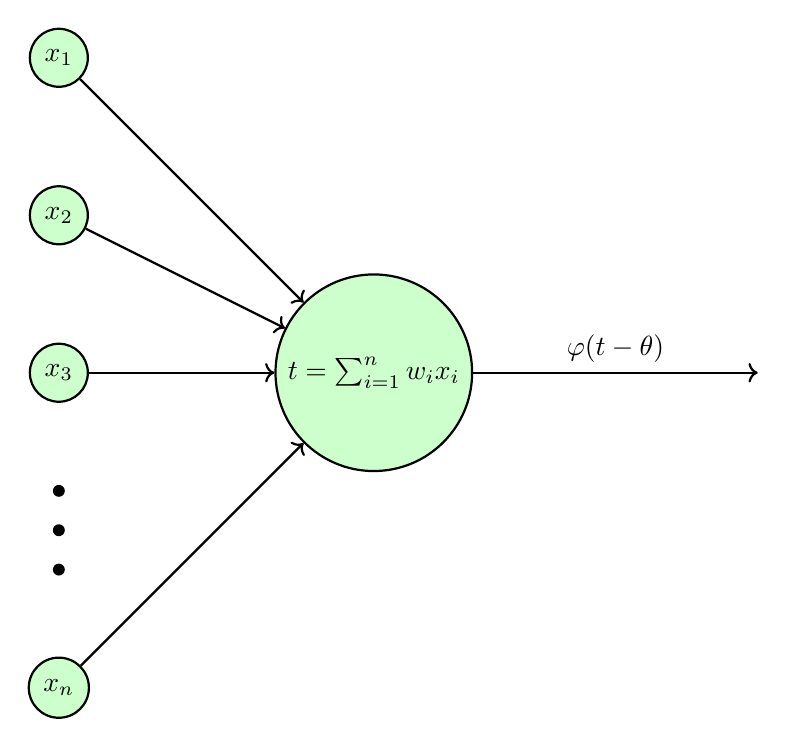
\begin{tikzpicture}[%
    dot/.style={circle,draw,thick,fill=green!20}
  ]
		\node at (5,0) (out) {};
		\node at (0,0) [dot] (neuron) {$t=\sum_{i=1}^{n}{w_ix_i}$}
			edge[->,thick] node[above]{$\varphi(t-\theta)$} (out);
		\node at (-4,4) [dot] {$x_1$}
			edge[->,thick] (neuron);
		\node at (-4,2) [dot] {$x_2$}
			edge[->,thick] (neuron);
		\node at (-4,0) [dot] {$x_3$}
			edge[->,thick] (neuron);
		\node at (-4,-4) [dot] {$x_n$}
			edge[->,thick] (neuron);
		\node at (-4,-1.5) [tokens=1] {};
		\node at (-4,-2) [tokens=1] {};
		\node at (-4,-2.5) [tokens=1] {};
	\end{tikzpicture}
	\end{center}
	\caption{Scheme of an artificial neuron}
	\label{fig_neuron}
\end{figure}



From chapter \ref{ss_nn_derivation_from_biology}, the
components and functioning of an artificial neuron can be
derived.
\newline\newline
In an artificial neuron the following happens:

\begin{enumerate}

  \item An artificial neuron is connected to other neurons
        or the direct value input via input connections,
        which are supposed to represent the synapses of the
        nerve cell (described in Figure \ref{fig_neuron}
        with $x_i$). These inputs can be discreet or
        continuous.\cite{nne_beck}

        If the data comes from other neurons, the weighting
        of the connection is additionally transferred to
        the value $\omega_i$ . Each connection of a neuron
        has an individual weighting. The greater the value
        of this weighting, the more important the
        transmitted value $x_i$ for the network output.

  \item The value and weight of each input connection is
        added by the transfer function $\sum_{i=1}^{n}w_ix_i$
        to calculate the net input value $t$.


  \item Every artificial neuron, like a nerve cell, has a
        threshold. An artificial neuron is a value
        $\theta$. The threshold $\theta$ is subtracted from
        the net input value $t$ to determine the activation
        potential of the neuron.

        The threshold can also be represented by the bias.
        The bias is a further input, which transmits the
        constant value 1 and as weighting the value
        $b=-\theta$.

        	\begin{figure}[H]
		\begin{center}
			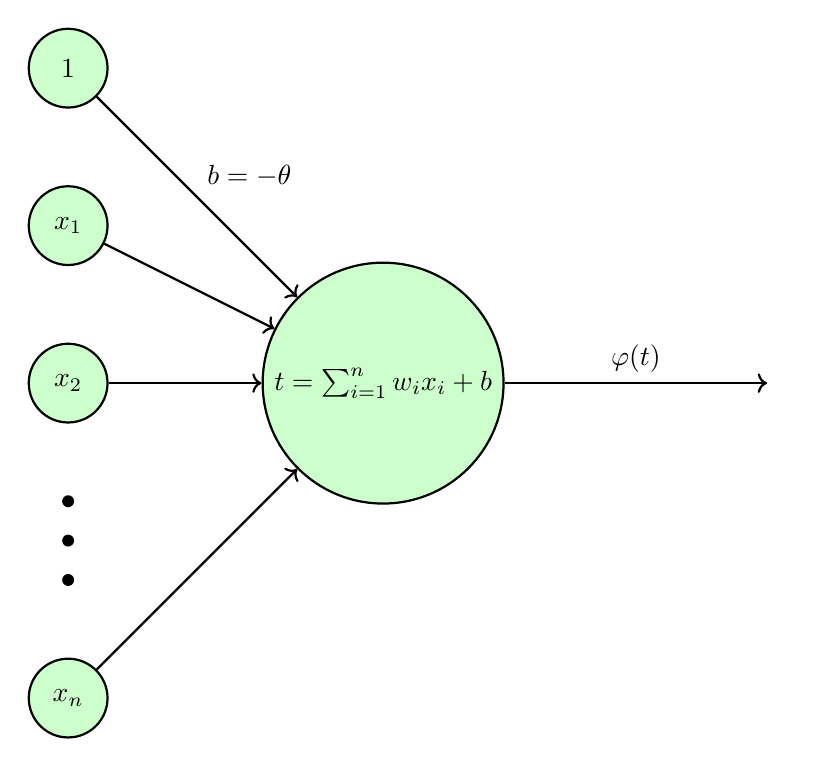
\begin{tikzpicture}[dot/.style={circle,draw,thick,fill=green!20,minimum size=1cm}]
				\node at (5,0) (out) {};
				\node at (0,0) [dot] (neuron) {$t=\sum_{i=1}^{n}{w_ix_i}+b$}
					edge[->,thick] node[above]{$\varphi(t)$} (out);
				\node at (-4,4) [dot] {$1$}
					edge[->,thick] node[anchor=south west]{$b=-\theta$} (neuron);
				\node at (-4,2) [dot] {$x_1$}
					edge[->,thick] (neuron);
				\node at (-4,0) [dot] {$x_2$}
					edge[->,thick] (neuron);
				\node at (-4,-4) [dot] {$x_n$}
					edge[->,thick] (neuron);
				\node at (-4,-1.5) [tokens=1] {};
				\node at (-4,-2) [tokens=1] {};
				\node at (-4,-2.5) [tokens=1] {};
			\end{tikzpicture}
		\end{center}
    \caption{An artificial neuron with bias}
    %\label{bn}
	\end{figure}



  \item The determined value of $t-\theta$ is used as an
        input in the activation function to determine the
        output of the neuron.

        From this process, the basic elements of a neuron
        can be determined:

        \begin{itemize}

          \item Weighting

          \item Threshold

          \item Transfer function

          \item Activation function

        \end{itemize}

\end{enumerate}
% }}}

% Construction of a neural network {{{
\subsubsection{Construction of a neural network}

\begin{figure}[H]
  \begin{center}
	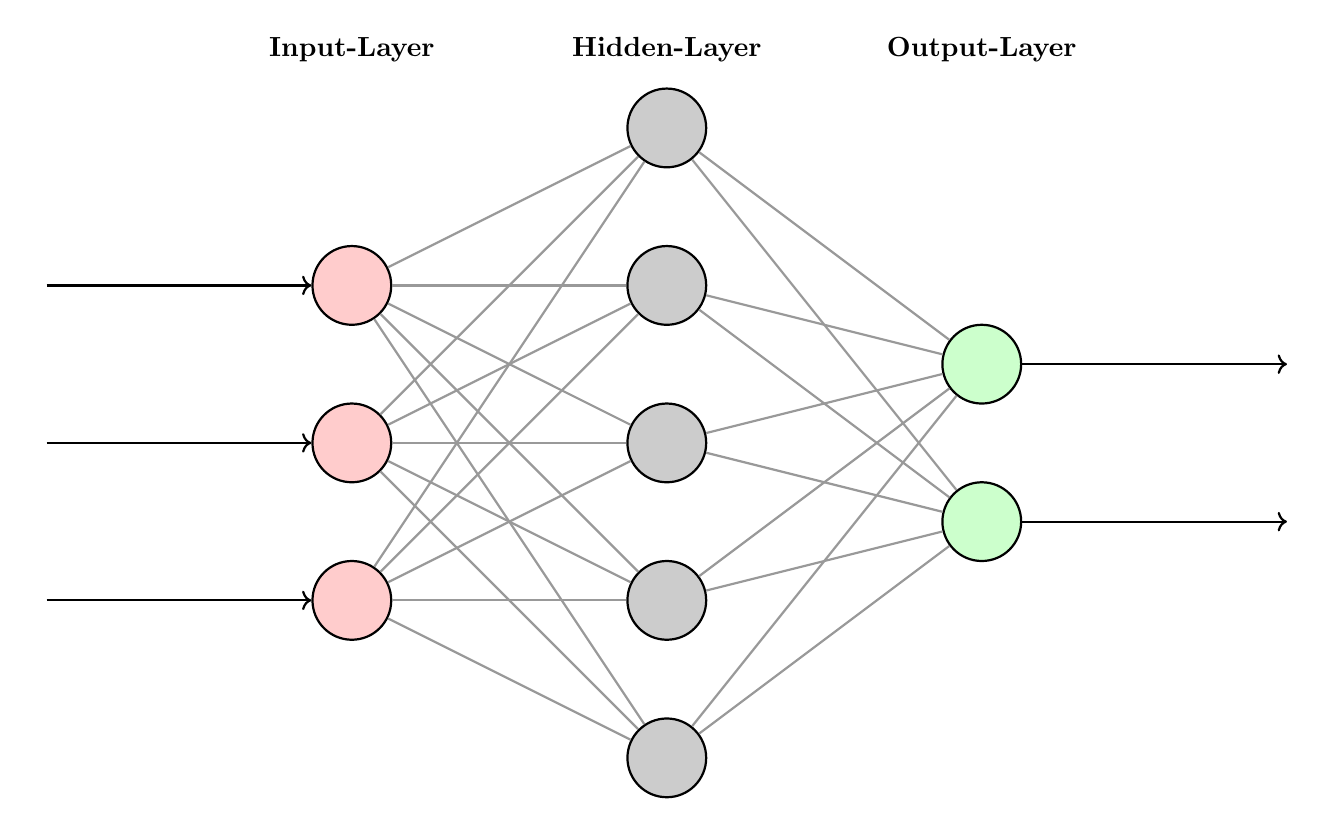
\begin{tikzpicture}[%
    dot/.style={circle,draw,thick,minimum size = 1cm}
  ]
		\node at(-4,5) {\textbf{Input-Layer}};
		\node at(0,5) {\textbf{Hidden-Layer}};
		\node at(4,5) {\textbf{Output-Layer}};

		\node at(8,1) (oo1) {};
		\node at(8,-1) (oo2) {};

		\node at (4,1) [dot,fill=green!20] (o1) {}
			edge[->,thick] (oo1);
		\node at (4,-1) [dot,fill=green!20] (o2) {}
			edge[->,thick] (oo2);

		\node at (0,4) [dot,fill=black!20] (h1) {}
			edge[thick,black!40] (o1)
			edge[thick,black!40] (o2);
		\node at (0,2) [dot,fill=black!20] (h2) {}
			edge[thick,black!40] (o1)
			edge[thick,black!40] (o2);
		\node at (0,0) [dot,fill=black!20] (h3) {}
			edge[thick,black!40] (o1)
			edge[thick,black!40] (o2);
		\node at (0,-2) [dot,fill=black!20] (h4) {}
			edge[thick,black!40] (o1)
			edge[thick,black!40] (o2);
		\node at (0,-4) [dot,fill=black!20] (h5) {}
			edge[thick,black!40] (o1)
			edge[thick,black!40] (o2);

		\node at (-4,2) [dot,fill=red!20] (i1) {}
			edge[thick,black!40] (h1)
			edge[thick,black!40] (h2)
			edge[thick,black!40] (h3)
			edge[thick,black!40] (h4)
			edge[thick,black!40] (h5);
		\node at (-4,0) [dot,fill=red!20] (i2) {}
			edge[thick,black!40] (h1)
			edge[thick,black!40] (h2)
			edge[thick,black!40] (h3)
			edge[thick,black!40] (h4)
			edge[thick,black!40] (h5);
		\node at (-4,-2) [dot,fill=red!20] (i3) {}
			edge[thick,black!40] (h1)
			edge[thick,black!40] (h2)
			edge[thick,black!40] (h3)
			edge[thick,black!40] (h4)
			edge[thick,black!40] (h5);

		\node at(-8,2) (ii1) {}
			edge[->,thick] (i1);
		\node at(-8,0) (ii2) {}
			edge[->,thick] (i2);
		\node at(-8,-2) (ii3) {}
			edge[->,thick] (i3);
	\end{tikzpicture}
  \end{center}
  \caption{Neural network with hidden layer}
  %\label{snn}
\end{figure}


% }}}


\subsection{Python}

...

\subsection{Tensorflow}

\subsection{Gym}

\subsection{Message Broker (RabbitMQ)}


\section{Application}

% Introduction {{{
Our goal was to make use of a lot of computing power in
order to train our agent to master an OpenAI Gym
Environment (cmp. \ref{s_openai_gym}). In this chapter we
will document how we tried to achieve this goal with our
distributed application.

% }}}

% The agent {{{
\subsection{The agent}

We programmed our agent as a neural network with the Keras
library, which has an API for high level, high abstraction
neural networks.

Keras uses Tensorflow as its backend for computations and
basically only provides a nicer abstraction of Tensorflow.

% example {{{
\begin{mdframed}[style=codebox]
\begin{lstlisting}[language=Python]
# a small example program using Keras
#
# API documentation at: https://keras.io/

# Sequential is the keras object representing a neural net-
# work
from keras.models import Sequential
# a neural net is comprised of layers connected with each
# other. The Dense object represents a layer
from keras.layers import Dense

# the neural net. This specific neural net has four layers
# (the input (size of 12), two hidden (both 64 artificial
# neurons) and the output layer (size of 4)). The input
# layer does not have to be specified since the input_dim
# parameter of the first layer automatically generates the
# input layer.
model = Sequential([
  Dense(64, activation='relu', input_dim=12 ),
  Dense(64, activation='relu'               ),
  Dense(4,  activation='softmax'            ),
])

# define how the model should learn and some other meta
# information for the training process (learning algorithm,
# optimizer, etc)
model.compile(
        optimizer = 'adam',
        loss      = 'categorical_crossentropy',
        metrics   = ['accuracy']
)

# generate a dummy data set with corresponding labels with
# 1000 entries for training
import numpy as np

data   = np.random.random((1000,12))
# generating the labels (either a 0 or a 1)
labels = np.random.randint(2, size=(1000, 1))

# training the model, iterating 10 times
model.train(data, labels, epochs=10)

# using the neural net to predict the label of a random
# data point
test   = np.random.random((1,12))

model.predict(test)
\end{lstlisting}
\end{mdframed}
% }}}
% }}}

\newpage

\subsection{Architecture}

This chapter will describe in detail how our application
is build, how it works and what we use to achieve
concurrency.

On a higher level our application is devided into two
distinct parts, the Executioner ($E$) and the Worker ($W$).

% Network {{{
\subsubsection{Network}

Instances of both, $E_i$ and $W_i$ communicate over a
message broker, in this case RabbitMQ (cmp.
\ref{s_message_broker}, \ref{s_rabbitmq}).

\begin{figure}[H]
\begin{center}
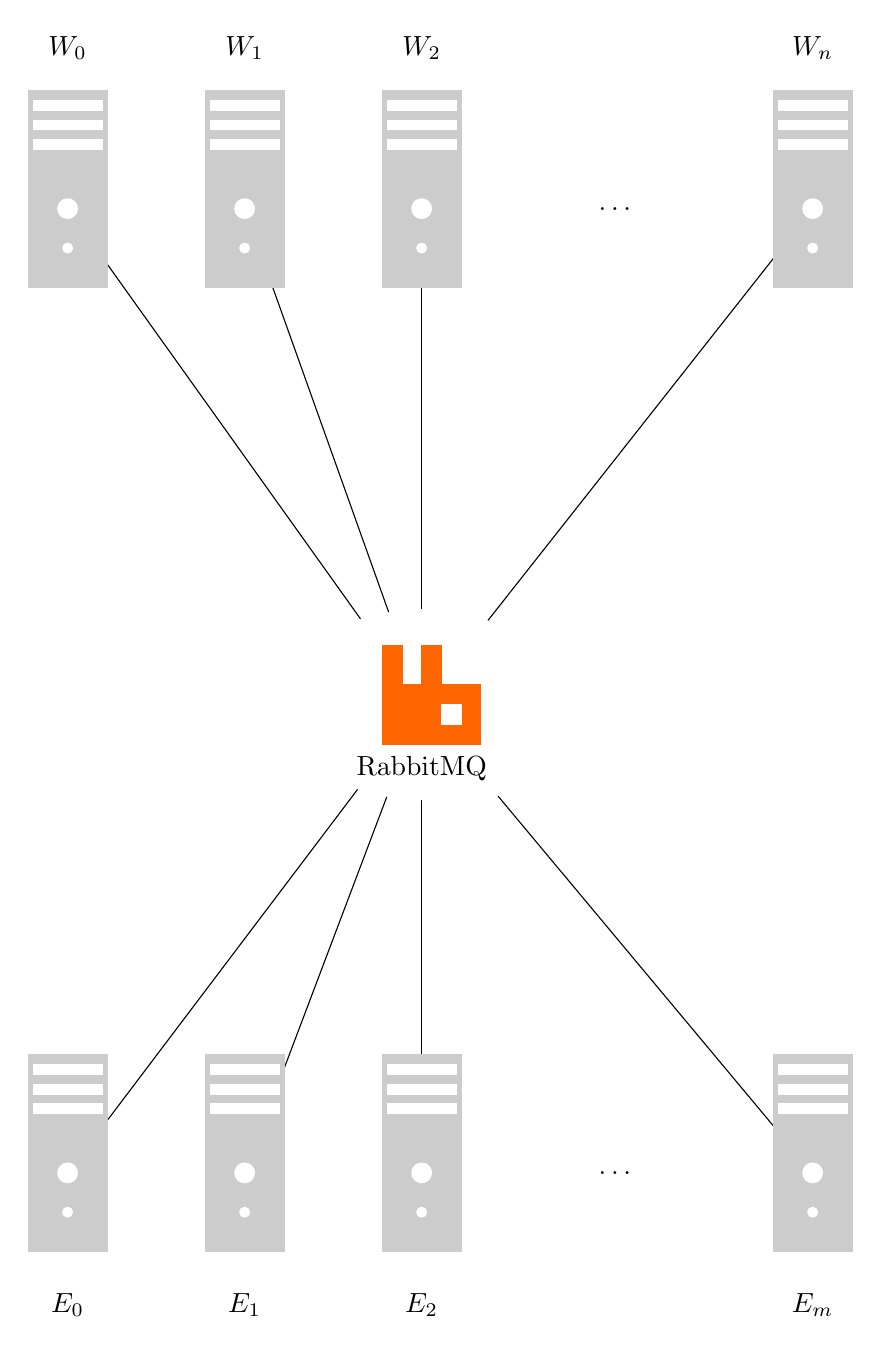
\begin{tikzpicture}

  \node[inner sep=15pt]
    at (0,0) (rmq) {};

  \node [label=$W_2$, inner ysep=50pt, above=4cm of rmq]
    (w_two) {};
  \draw[-{Stealth[color=white,length=10mm]}]
    (w_two.center) -- (rmq);
  \PCIcon{w_two}{scale=.25}

  \node [label=$W_1$, inner ysep=50pt, left =2cm of w_two]
    (w_one)   {};
  \draw[-{Stealth[color=white,length=10mm]}]
    (w_one.center) -- (rmq);
  \PCIcon{w_one}{scale=.25}

  \node [label=$W_0$, inner ysep=50pt, left =2cm of w_one]
    (w_zero)   {};
  \draw[-{Stealth[color=white,length=10mm]}]
    (w_zero.center) -- (rmq);
  \PCIcon{w_zero}{scale=.25}

  \node [right=2cm of w_two] (w_dots) {\dots};

  \node [label=$W_n$, inner ysep=50pt, right=2cm of w_dots]
    (w_n) {};
  \draw[-{Stealth[color=white,length=10mm]}]
    (w_n.center) -- (rmq);
  \PCIcon{w_n}{scale=.25}


  \node [label={below:$E_2$}, inner ysep=40pt,
    below=4cm of rmq]
    (e_two) {}
    edge[-{Stealth[color=white,length=10mm]}] (rmq);
  \PCIcon{e_two}{scale=.25}

  \node [label={below:$E_1$}, inner ysep=40pt,
    left =2cm of e_two]
    (e_one)   {}
    edge[-{Stealth[color=white,length=10mm]}] (rmq);
  \PCIcon{e_one}{scale=.25}

  \node [label={below:$E_0$}, inner ysep=40pt,
    left =2cm of e_one]
    (e_zero)   {}
    edge[-{Stealth[color=white,length=10mm]}] (rmq);
  \PCIcon{e_zero}{scale=.25}

  \node [right=2cm of e_two] (e_dots) {\dots};

  \node [label={below:$E_m$}, inner ysep=40pt,
    right=2cm of e_dots]
    (e_n) {}
    edge[-{Stealth[color=white,length=12mm]}] (rmq);
  \PCIcon{e_n}{scale=.25}


  \node[label={below:RabbitMQ},inner ysep=15pt]
    at (0,0) {};
  \RabbitMQ{rmq}{scale=.25}

\end{tikzpicture}
\end{center}
\caption{Architecture of our Application on the network
  level}
\end{figure}

% }}}

% Executioner {{{
\subsubsection{Executioner}

% }}}

% Worker {{{
\subsubsection{Worker}

here comes the data sanitation part

% }}}

\subsubsection{Queues}


\subsection{Results}

\subsection{Where to go}

(dynamic data generation, loadbalancing, further optimizations
like thread pool exec in worker (not spawning so often),
destroying the bottleneck in executioner (data parsing))


\printindex
\Urlmuskip 0mu plus 1mu\relax
\bibliography{wpfvs_bib}
\end{document}
